\documentclass[12pt,a4paper,twoside]{article}

% ------------------------------------------------------------------ pacotes
\usepackage[T1]{fontenc}
\usepackage[utf8]{inputenc}
\usepackage[brazil]{babel}
\usepackage{lmodern}
\usepackage{microtype}
\usepackage[a4paper,margin=2.5cm]{geometry}
\usepackage{amsmath,amssymb,amsthm,bm}
\usepackage{graphicx}
\usepackage{booktabs,array,tabularx,multirow}
\usepackage{caption,subcaption}
\usepackage{xcolor}
\usepackage{tikz}
\usetikzlibrary{arrows.meta,angles,quotes,calc,patterns,babel}
\usepackage[output-decimal-marker={,}, group-separator={.}, range-phrase={ a }, list-final-separator={ e }, list-pair-separator={ e }, list-separator={; }]{siunitx}
\usepackage{enumitem}
\usepackage{csquotes}
\usepackage[style=abnt,backend=biber]{biblatex}
\addbibresource{referencias.bib}
\usepackage{fancyhdr}
\usepackage{setspace}
\usepackage{longtable}
\usepackage{indentfirst}
\setlength{\parindent}{1.5em}
\onehalfspacing
\pagestyle{fancy}
\fancyhf{}
\fancyhead[LE,RO]{Relatório Parcial}
\fancyhead[RE,LO]{PMR3220 - Projeto de Mecanismos}
\fancyfoot[LE,RO]{\thepage}
\fancyfoot[RE,LO]{\textit{\nouppercase{\leftmark}}}
\renewcommand{\sectionmark}[1]{\markboth{#1}{}}
\renewcommand{\headrulewidth}{0.4pt}
\renewcommand{\footrulewidth}{0.4pt}
\usepackage[hidelinks]{hyperref}
\usepackage[brazilian,capitalise,noabbrev]{cleveref}
\usepackage{listings}

\lstset{basicstyle=\ttfamily\footnotesize, breaklines=true, frame=single,
        literate={á}{{\'a}}1 {ã}{{\~a}}1 {é}{{\'e}}1 {ç}{{\c{c}}}1 {õ}{{\~o}}1 {í}{{\'i}}1 {ó}{{\'o}}1}

% Arquivo gerado automaticamente por scripts/gera_valores_tex.py -- nao editar
\newcommand{\Qx}{67{,}4}
\newcommand{\Qy}{\ensuremath{-}97{,}8}
\newcommand{\Nx}{\ensuremath{-}6{,}6}
\newcommand{\Ny}{\ensuremath{-}24{,}6}
\newcommand{\Cx}{\ensuremath{-}7{,}6}
\newcommand{\Cy}{\ensuremath{-}14{,}0}
\newcommand{\Lx}{\ensuremath{-}28{,}4}
\newcommand{\Ly}{\ensuremath{-}24{,}3}
\newcommand{\Px}{39{,}6}
\newcommand{\Py}{\ensuremath{-}419{,}0}
\newcommand{\rCL}{23{,}2}
\newcommand{\rCQ}{112{,}5}
\newcommand{\rQN}{104{,}1}
\newcommand{\rLN}{21{,}8}
\newcommand{\mumin}{42{,}5}
\newcommand{\mumax}{89{,}9}
\newcommand{\grashof}{não satisfaz}
\newcommand{\grashofs}{21{,}8}
\newcommand{\grashofp}{23{,}2}
\newcommand{\grashofq}{104{,}1}
\newcommand{\grashofl}{112{,}5}
\newcommand{\grashofsl}{134{,}3}
\newcommand{\grashofpq}{127{,}3}
\newcommand{\grashofsinal}{>}
\newcommand{\ciOx}{1{,}9}
\newcommand{\ciOy}{\ensuremath{-}24{,}7}
\newcommand{\ciFx}{\ensuremath{-}32{,}3}
\newcommand{\ciFy}{\ensuremath{-}21{,}0}
\newcommand{\phimax}{132{,}0}
\newcommand{\frA}{307}
\newcommand{\phiA}{0{,}0}
\newcommand{\frB}{390}
\newcommand{\phiB}{51{,}7}
\newcommand{\frC}{423}
\newcommand{\phiC}{97{,}2}
\newcommand{\frD}{456}
\newcommand{\phiD}{131{,}9}
\newcommand{\precA}{307}
\newcommand{\precB}{423}
\newcommand{\precC}{456}
\newcommand{\cheque}{390}
\newcommand{\phicheque}{51{,}7}
\newcommand{\errcheque}{0{,}7}
\newcommand{\JPmin}{356}
\newcommand{\JPmax}{367}
\newcommand{\JPvar}{3}
\newcommand{\Jx}{2{,}7}
\newcommand{\Jy}{\ensuremath{-}62{,}2}
\newcommand{\deslO}{60}
\newcommand{\rmaxelo}{112{,}5}
\newcommand{\dalphaA}{\ensuremath{-}97{,}2}
\newcommand{\dalphaB}{\ensuremath{-}131{,}9}
\newcommand{\ddeltaAx}{16{,}7}
\newcommand{\ddeltaAy}{\ensuremath{-}37{,}2}
\newcommand{\ddeltaBx}{2{,}0}
\newcommand{\ddeltaBy}{\ensuremath{-}59{,}9}
\newcommand{\dbetaA}{\ensuremath{-}88{,}0}
\newcommand{\dbetaB}{\ensuremath{-}116{,}0}
\newcommand{\dgamA}{\ensuremath{-}8{,}0}
\newcommand{\dgamB}{\ensuremath{-}40{,}0}
\newcommand{\dWx}{75{,}0}
\newcommand{\dWy}{\ensuremath{-}83{,}8}
\newcommand{\dZx}{\ensuremath{-}67{,}4}
\newcommand{\dZy}{97{,}8}
\newcommand{\dUx}{21{,}8}
\newcommand{\dUy}{\ensuremath{-}0{,}3}
\newcommand{\dSx}{6{,}6}
\newcommand{\dSy}{24{,}6}
\newcommand{\tabelaposes}{234 $\dagger$ & 15{,}4 & 2{,}1 & 1{,}4 & \ensuremath{-}70{,}7 & \ensuremath{-}413{,}1 & 359 \\
307 $\star$ & 0{,}0 & 0{,}0 & 0{,}0 & 39{,}6 & \ensuremath{-}419{,}0 & 359 \\
390 $\circ$ & 51{,}7 & 17{,}3 & \ensuremath{-}12{,}9 & \ensuremath{-}287{,}1 & \ensuremath{-}303{,}5 & 367 \\
423 $\star$ & 97{,}2 & 16{,}7 & \ensuremath{-}37{,}2 & \ensuremath{-}404{,}0 & \ensuremath{-}24{,}3 & 356 \\
456 $\star$ & 131{,}9 & 2{,}0 & \ensuremath{-}59{,}9 & \ensuremath{-}336{,}3 & 190{,}5 & 361 \\
561 $\dagger$ & 155{,}1 & \ensuremath{-}30{,}4 & \ensuremath{-}60{,}4 & \ensuremath{-}242{,}5 & 303{,}1 & 345 \\}
\newcommand{\tabelacombos}{307, 423, 456 & 390 & 0{,}71 & 42{,}5 \\
307, 390, 456 & 423 & 0{,}93 & 38{,}6 \\
307, 390, 423 & 456 & 0{,}99 & 32{,}2 \\}
\newcommand{\mUmA}{9{,}88}
\newcommand{\aUmA}{0{,}207}
\newcommand{\IUmA}{0{,}202}
\newcommand{\mDoisA}{5{,}44}
\newcommand{\bxDoisA}{0{,}258}
\newcommand{\byDoisA}{0{,}031}
\newcommand{\IDoisA}{0{,}172}
\newcommand{\mUmB}{7{,}88}
\newcommand{\aUmB}{0{,}215}
\newcommand{\IUmB}{0{,}165}
\newcommand{\mDoisB}{4{,}22}
\newcommand{\bxDoisB}{0{,}259}
\newcommand{\byDoisB}{0{,}031}
\newcommand{\IDoisB}{0{,}133}
\newcommand{\mUmS}{8{,}00}
\newcommand{\mDoisS}{4{,}88}
\newcommand{\massaOrtese}{2{,}43}
\newcommand{\tabelaortese}{coxa & hastes laterais Al 6061-T6 (2x) & 0{,}216 & (0{,}200; 0{,}000) \\
perna & hastes laterais Al 6061-T6 (2x) & 0{,}243 & (0{,}225; 0{,}000) \\
coxa & braçadeira proximal PP & 0{,}131 & (0{,}100; 0{,}000) \\
coxa & braçadeira distal PP & 0{,}131 & (0{,}300; 0{,}000) \\
perna & braçadeira PP & 0{,}131 & (0{,}150; 0{,}000) \\
perna & palmilha PP + estribo & 0{,}181 & (0{,}450; 0{,}125) \\
coxa & articulação do joelho (aço AISI 304) & 0{,}200 & (0{,}400; 0{,}000) \\
coxa & atuador do joelho (motor + redutor) & 1{,}200 & (0{,}400; 0{,}000) \\}
\newcommand{\tabelatorques}{final I & 80 & 6{,}2 & 13{,}5 \\
final I & 60 & 4{,}7 & 10{,}5 \\
final II & 80 & 40{,}0 & 2{,}8 \\
final II & 60 & 32{,}1 & 2{,}2 \\}
\newcommand{\tabelacinematica}{final I & 9{,}5 & 103{,}0 & 112{,}5 & 14{,}6 & 158{,}6 & 173{,}2 \\
final II & 93{,}8 & 9{,}2 & 103{,}0 & 144{,}4 & 14{,}2 & 158{,}6 \\}
\newcommand{\tqImax}{6{,}2}
\newcommand{\tjImax}{13{,}5}
\newcommand{\tqIImax}{40{,}0}
\newcommand{\tjIImax}{2{,}8}
\newcommand{\wmaxII}{93{,}8}
\newcommand{\wmaxI}{112{,}5}
\newcommand{\repQ}{1{,}645}
\newcommand{\repJ}{1{,}645}
\newcommand{\repmgb}{1{,}645}


\newcommand{\ve}[1]{\bm{#1}}
% --- notacao do metodo matricial (PMR3220) ---
\DeclareMathOperator{\sen}{sen}
\newcommand{\rv}[2]{{}^{#1}\mathbf{r}_{#2}}          % vetor posicao do ponto #2 na base #1
\newcommand{\rvd}[2]{{}^{#1}\dot{\mathbf{r}}_{#2}}
\newcommand{\rvdd}[2]{{}^{#1}\ddot{\mathbf{r}}_{#2}}
\newcommand{\vv}[2]{{}^{#1}\mathbf{v}_{#2}}
\newcommand{\Rmd}[2]{[{}^{#1}\dot R_{#2}]}             % derivadas da matriz de rotacao
\newcommand{\Rmdd}[2]{[{}^{#1}\ddot R_{#2}]}
\newcommand{\Et}{\tilde{\mathbf k}}                   % matriz antissimetrica de k no plano
\newcommand{\Rm}[2]{[{}^{#1}R_{#2}]}                 % matriz de rotacao
\newcommand{\Rot}[2]{\mathrm{Rot}(#1,\,#2)}
\newcommand{\Jm}[1]{[J_{#1}]}
\newcommand{\e}{\mathrm{e}}
\newcommand{\dd}{\,\mathrm{d}}
\newtheorem{hipotese}{Hipótese}
\captionsetup{font=small,labelsep=colon}
\numberwithin{equation}{section}

% ------------------------------------------------------------------ capa
\begin{document}
\begin{titlepage}
  \centering
  {\Large\bfseries ESCOLA POLITÉCNICA DA UNIVERSIDADE DE SÃO PAULO\par}
  \vspace{1.2cm}
  {\large\bfseries PMR3220 - Projeto de Mecanismos\par}
  \vspace{0.8cm}
  Prof. Dr. Ricardo Cury Ibrahim\par
  Prof. Dr. Tarcisio Antonio Hess Coelho\par
  \vspace{0.9cm}
  {\bfseries Grupo C\par}
  \vspace{0.5cm}
  \begin{spacing}{1.6}
  André Neme Benedetti - NUSP\par
  André Tsukassa Nishimoto - NUSP\par
  Felipe Wassmer Magina - NUSP\par
  Júlio Cesar de Andrade Oliveira - NUSP\par
  Lucas Sung Il Hong - NUSP\par
  Matheus Moreira de Sousa - NUSP\par
  Matheus Paixão de Sousa - NUSP\par
  Pedro Henrique Brasileiro de Jesus - NUSP\par
  \end{spacing}
  \vspace{0.7cm}
  {\LARGE Relatório Parcial\par}
  \vspace{0.3cm}
  {\bfseries Prótese e órtese de membro inferior\par}
  \vspace{0.8cm}
  
\includegraphics[width=4.2cm]{figuras/logo_poli_usp.png}\par
  \vfill
  {\large\bfseries São Paulo, 7 de outubro de 2026\par}
\end{titlepage}

\pagenumbering{roman}
\listoffigures
\clearpage
\listoftables
\clearpage
\tableofcontents
\clearpage
\pagenumbering{arabic}
\setcounter{page}{5}

\section{Introdução}

O movimento do membro inferior humano resulta da interação entre diferentes segmentos
e articulações, sendo o joelho particularmente importante para a mobilidade entre a
coxa e a perna. Entretanto, seu movimento relativo não pode ser rigorosamente
representado por uma simples junta de revolução: no plano sagital, os côndilos
femorais rolam e deslizam sobre o platô tibial, de modo que o centro instantâneo de
rotação (CIR) descreve uma trajetória -- a \emph{centroide} -- em vez de permanecer fixo
\cite{menschik1974,oconnor1989,dathe2016}. Desde \textcite{menschik1974}, essa cinemática
é modelada por um quadrilátero articulado cruzado, formado pelas fibras isométricas
dos ligamentos cruzados anterior (LCA) e posterior (LCP) e pelos segmentos ósseos que
unem suas inserções \cite{oconnor1989,zavatsky1992}.

Nesse contexto, o projeto de próteses e órteses constitui uma aplicação relevante da
teoria de mecanismos, permitindo reproduzir ou auxiliar movimentos do membro inferior
em situações de amputação ou de comprometimento da capacidade motora -- por exemplo,
após um acidente grave, um acidente vascular cerebral (AVC) ou uma lesão por esforço
intenso. Este trabalho aborda a aplicação de mecanismos articulados a esses problemas
em duas partes, propostas no enunciado da disciplina (\cref{fig:enunciado}):

Este documento trata da primeira parte do trabalho: a síntese dimensional de um
quadrilátero articulado plano cujo acoplador (conjunto perna--pé artificial) reproduza o
movimento relativo entre a perna e a coxa, medido experimentalmente em um integrante do
grupo, e a construção de uma maquete para avaliar qualitativamente o funcionamento
(\cref{fig:enunciado}).

\begin{figure}[htbp]
  \centering
  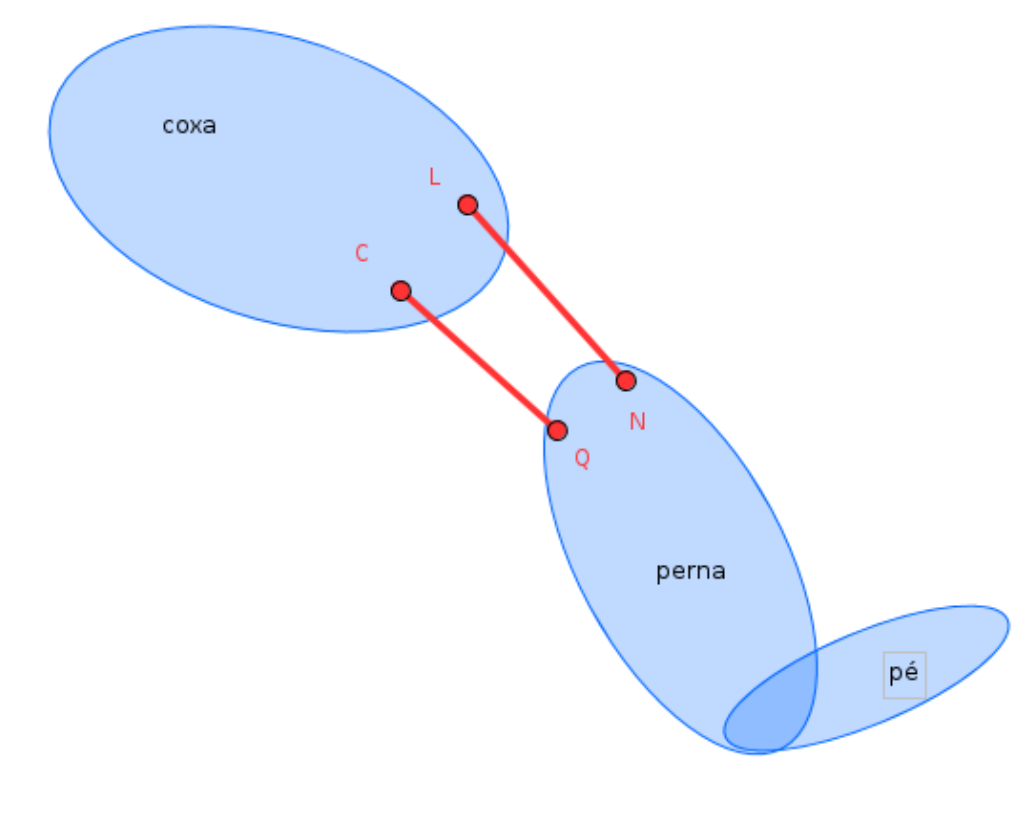
\includegraphics[width=0.42\textwidth]{figuras/enunciado_fig1.png}
  \caption{Diagrama cinemático do enunciado: pivôs $C$ e $L$ na coxa e $Q$ e $N$ na perna.}
  \label{fig:enunciado}
\end{figure}

\section{Objetivos}

\begin{itemize}
  \item Desenvolver a síntese dimensional de um mecanismo quadrilátero articulado,
  capaz de reproduzir de forma aproximada o movimento relativo entre a coxa e o
  conjunto perna--pé de uma prótese de membro inferior.
  \item Determinar as dimensões e as posições das articulações do mecanismo, utilizando
  como referência as posições do membro inferior obtidas experimentalmente.
  \item Construir uma maquete que permita avaliar qualitativamente o funcionamento do
  mecanismo sintetizado.
\end{itemize}

Em todas as deduções, os passos intermediários são mostrados, de modo que os
resultados possam ser reproduzidos à mão. Os cálculos foram implementados em Python
(NumPy e Matplotlib), e os valores numéricos citados no texto são lidos
automaticamente dos resultados (\cref{sec:anexos}).

\section{Fundamentação teórica}\label{cap:teoria1}

\subsection{Notação}\label{sec:notacao}

A modelagem cinemática segue o \emph{método matricial} adotado na disciplina, baseado em
matrizes de rotação e na mudança de base de pontos. A cada elo $i$ associa-se uma base (sistema de referência)
$O_iX_iY_iZ_i$, de versores $\mathbf i_i$, $\mathbf j_i$, $\mathbf k_i$; a base $0$ é fixa. As
convenções são:
\begin{itemize}
  \item $\rv{A}{P}$: vetor posição do ponto $P$ escrito na base $A$ (o sobrescrito à esquerda
  indica a base);
  \item $\Rm{A}{B} = [\,{}^{A}\mathbf i_B,\ {}^{A}\mathbf j_B,\ {}^{A}\mathbf k_B\,]$: matriz de rotação
  cujas colunas são os versores da base $B$ escritos na base $A$, com
  $\Rm{B}{A} = \Rm{A}{B}^{-1} = \Rm{A}{B}^{\mathsf T}$;
  \item rotação simples de ângulo $\gamma$ em torno do eixo $z_B$ (movimento plano):
  \begin{equation}
    \Rm{A}{B} = \Rot{\gamma}{z_B} =
    \begin{bmatrix} \cos\gamma & -\sen\gamma & 0\\ \sen\gamma & \cos\gamma & 0\\ 0 & 0 & 1 \end{bmatrix},
    \qquad
    \begin{aligned}
      \mathbf i_B &= \cos\gamma\,\mathbf i_A + \sen\gamma\,\mathbf j_A,\\
      \mathbf j_B &= -\sen\gamma\,\mathbf i_A + \cos\gamma\,\mathbf j_A,\\
      \mathbf k_B &= \mathbf k_A;
    \end{aligned}
  \end{equation}
  no plano, usa-se apenas o bloco $2\times2$ superior;
  \item mudança de base de um ponto: se $\rv{B}{P}$ são as coordenadas de $P$ na base $B$ e
  $\rv{A}{O_B}$ a posição da origem de $B$ na base $A$, então
  \begin{equation}
    \rv{A}{P} = \Rm{A}{B}\,\rv{B}{P} + \rv{A}{O_B} ;
    \label{eq:mudancabase}
  \end{equation}
  para uma cadeia de bases $0, 1, 2$, aplica-se \eqref{eq:mudancabase} duas vezes, de dentro para fora:
  \begin{equation}
    \rv{0}{P} = \rv{0}{O_1} + \Rm{0}{1}\Big(\rv{1}{O_2} + \Rm{1}{2}\,\rv{2}{P}\Big),
    \qquad
    \Rm{0}{2} = \Rm{0}{1}\,\Rm{1}{2} ;
    \label{eq:cadeia}
  \end{equation}
  \item derivada no tempo de uma rotação plana: de $\Rm{A}{B} = \Rot{\gamma}{z}$,
  \begin{gather}
    \Rmd{A}{B} = \dot\gamma\begin{bmatrix} -\sen\gamma & -\cos\gamma \\ \cos\gamma & -\sen\gamma \end{bmatrix}
             = \dot\gamma\,\Rm{A}{B}\,\Et ,
    \qquad
    \Et = \begin{bmatrix} 0 & -1 \\ 1 & 0 \end{bmatrix},
    \label{eq:derivR}\\
    \Rmdd{A}{B} = \ddot\gamma\,\Rm{A}{B}\,\Et - \dot\gamma^2\,\Rm{A}{B} ;
  \end{gather}
  \item abreviações: $c_i = \cos\theta_i$, $s_i = \sen\theta_i$, $c_{ij} = \cos(\theta_i+\theta_j)$,
  $s_{ij} = \sen(\theta_i+\theta_j)$; o ângulo $\theta_i$ da junta $i$ é medido do eixo $X_{i-1}$ ao
  eixo $X_i$ (ângulo \emph{relativo}), positivo no sentido anti-horário;
  \item produto vetorial na forma matricial: $\mathbf a \times \mathbf b = \tilde{\mathbf a}\,\mathbf b$, com
  $\tilde{\mathbf a} = \begin{bmatrix} 0 & -a_z & a_y\\ a_z & 0 & -a_x\\ -a_y & a_x & 0\end{bmatrix}$.
\end{itemize}

\subsection{Síntese do tipo e mobilidade: o quadrilátero articulado}

A escolha do tipo de mecanismo parte da mobilidade desejada. O movimento relativo
perna--coxa no plano sagital é comandado por uma única variável (a flexão do joelho), de
modo que o mecanismo deve ter um grau de liberdade, $M = 1$. Pelo critério de Grübler para
mecanismos planos,
\begin{equation}
  M = 3(n-1) - 2j_1 - j_2 ,
\end{equation}
em que $n$ é o número de elos (incluindo o fixo), $j_1$ o de juntas de um grau de liberdade
(revolução ou prismática) e $j_2$ o de juntas de dois graus de liberdade. Usando apenas
juntas de revolução ($j_2 = 0$), $M = 1$ exige $3n - 2j_1 = 4$. A menor solução com $n > 2$ é
$n = 4$, $j_1 = 4$:
\begin{equation}
  M = 3(4-1) - 2\cdot 4 - 0 = 1 ,
\end{equation}
ou seja, o \emph{quadrilátero articulado}. A alternativa $n = 2$, $j_1 = 1$ (uma única junta de
revolução) também tem $M = 1$, mas impõe à perna um centro de rotação fixo, o que não
reproduz o movimento do joelho (\cref{sec:processamento}). A solução seguinte,
$n = 6$ e $j_1 = 7$, levaria a mecanismos de seis barras, mais complexos que o necessário.

No joelho protético (\cref{fig:enunciado}) o elo fixo é a coxa (pivôs $C$ e $L$),
as manivelas/balancins são $CQ$ e $LN$, e o \emph{acoplador} é a perna (pivôs $Q$ e $N$),
ao qual se fixa rigidamente o pé. Como o acoplador executa um movimento plano geral,
seu CIR relativo à coxa -- o polo $I_{13}$ -- é, pelo teorema de Aronhold--Kennedy, a
intersecção das retas $CQ$ e $LN$ e se desloca à medida que o joelho flexiona, tal como
no joelho natural \cite{norton2010,radcliffe1994}. Joelhos protéticos de quatro barras
exploram essa propriedade: com o CIR alto e posterior na extensão, obtém-se
estabilidade voluntária na fase de apoio; com o CIR migrando na flexão, obtém-se
encurtamento aparente da perna na fase de balanço \cite{radcliffe1994}.

A condição de Grashof classifica o tipo de movimento possível. Sendo $s$ e $l$ os
comprimentos do menor e do maior elo e $p$, $q$ os demais,
\begin{equation}
  s + l \le p + q \quad\Longrightarrow\quad \text{pelo menos um elo dá voltas completas.}
  \label{eq:grashof}
\end{equation}
Na prótese, a flexão útil está limitada a cerca de \SI{120}{\degree}; logo, um mecanismo
não Grashof (triplo balancim) é aceitável, desde que nenhuma configuração de ponto
morto ocorra dentro dessa faixa. A qualidade da transmissão de forças é avaliada pelo
ângulo de transmissão $\mu$ -- ângulo agudo entre o acoplador e o balancim de saída --,
recomendando-se $\mu \ge \SI{30}{\degree}$ \cite{norton2010}.

\subsection{Bases e análise de posição do quadrilátero (cadeia fechada)}\label{sec:cadeia_fechada}

A \cref{fig:quadrilatero} mostra as bases adotadas, seguindo a convenção da
\cref{sec:notacao}. A base $0$ (fixa) está presa à coxa, com origem no centro do joelho em
extensão, $X_0$ para a frente (anterior) e $Y_0$ para cima (proximal). As bases $1$, $2$ e $3$
estão presas, respectivamente, ao elo $CQ$ (origem em $C$, $X_1$ ao longo de $CQ$), ao
acoplador (origem em $Q$, $X_2$ ao longo de $QN$) e ao elo $LN$ (origem em $L$, $X_3$ ao longo
de $LN$). A base $4$ também está presa à perna, com origem no ponto $J$ (ponto médio dos
marcadores 5 e 6, logo abaixo do joelho) e eixos paralelos aos da base $0$ com o membro
estendido (é a base em que se fazem as medições). Todas as bases, portanto, são solidárias a
uma peça: a base $0$ à coxa, as bases $1$ e $3$ às barras $CQ$ e $LN$ e as bases $2$ e $4$ à
perna, que é o acoplador. Os
comprimentos são $\ell_0 = \overline{CL}$, $\ell_1 = \overline{CQ}$, $\ell_2 = \overline{QN}$ e
$\ell_3 = \overline{LN}$.

\begin{figure}[htbp]
  \centering
  \begin{tikzpicture}[scale=1.35, >=Stealth]
    \coordinate (C) at (0,0);
    \coordinate (L) at (3,0.6);
    \coordinate (Q) at ({1.6*cos(115)},{1.6*sin(115)});
    \coordinate (N) at ($(L)+({2.4*cos(128)},{2.4*sin(128)})$);
    \draw[thick] (C) -- node[left, pos=0.6] {$\ell_1$} (Q) -- node[above left, pos=0.6] {$\ell_2$} (N) -- node[right] {$\ell_3$} (L);
    \draw[thick,dashed,gray] (C) -- node[below] {$\ell_0$} (L);
    \foreach \p in {C,Q,N,L} \draw[fill=white] (\p) circle (0.06);
    \node[below left] at (C) {$C$}; \node[below right] at (L) {$L$};
    \node[left] at (Q) {$Q$}; \node[above right] at (N) {$N$};
    % base 0
    \draw[->,thick] (-1.2,-0.8) -- (-0.4,-0.8) node[below] {$X_0$};
    \draw[->,thick] (-1.2,-0.8) -- (-1.2,0) node[left] {$Y_0$};
    % base 1
    \draw[->,teal] (C) -- ($(C)!0.45!(Q)$) node[right=2pt] {$X_1$};
    \draw[dashed,blue] (C) -- (1,0) coordinate (Ce);
    \pic[draw,->,blue,"$\theta_1$",angle radius=0.5cm,angle eccentricity=1.45] {angle=Ce--C--Q};
    % base 2
    \coordinate (Qe) at ($(Q)!-0.5!(C)$);
    \draw[dashed,blue] (Q) -- (Qe);
    \draw[->,teal] (Q) -- ($(Q)!0.3!(N)$) node[below] {$X_2$};
    \pic[draw,->,blue,"$\theta_2$",angle radius=0.45cm,angle eccentricity=1.5] {angle=N--Q--Qe};
    % base 3
    \draw[dashed,blue] (L) -- ($(L)+(0.8,0.16)$) coordinate (Le);
    \draw[->,teal] (L) -- ($(L)!0.25!(N)$) node[left] {$X_3$};
    \pic[draw,->,blue,"$\theta_3$",angle radius=0.45cm,angle eccentricity=1.5] {angle=Le--L--N};
    \node[gray] at (0.4,2.8) {perna (acoplador)};
    \node[gray] at (1.5,-0.6) {coxa (elo fixo 0)};
  \end{tikzpicture}
  \caption{Quadrilátero articulado do joelho: bases, ângulos e comprimentos (a base $1$ e a
  base $3$ têm os ângulos medidos a partir de $X_0$; $\theta_2$ é medido a partir de $X_1$).}
  \label{fig:quadrilatero}
\end{figure}

As matrizes de rotação e as origens das bases são
\begin{gather}
  \Rm{0}{1} = \begin{bmatrix} c_1 & -s_1 \\ s_1 & c_1 \end{bmatrix},\quad
  \Rm{1}{2} = \begin{bmatrix} c_2 & -s_2 \\ s_2 & c_2 \end{bmatrix},\quad
  \Rm{0}{3} = \begin{bmatrix} c_3 & -s_3 \\ s_3 & c_3 \end{bmatrix},\\
  \rv{0}{O_1} = \rv{0}{C},\qquad \rv{1}{O_2} = \begin{bmatrix} \ell_1 \\ 0 \end{bmatrix},\qquad \rv{0}{O_3} = \rv{0}{L},
\end{gather}
com $\rv{2}{N} = [\ell_2\ \ 0]^{\mathsf T}$ e $\rv{3}{N} = [\ell_3\ \ 0]^{\mathsf T}$. O ponto $N$ pertence
simultaneamente ao ramo $0\text{--}1\text{--}2$ e ao ramo $0\text{--}3$ da cadeia. Pelo ramo
$0\text{--}1\text{--}2$, aplica-se \eqref{eq:cadeia} de dentro para fora:
\begin{align*}
  \rv{1}{N} &= \rv{1}{O_2} + \Rm{1}{2}\,\rv{2}{N}
            = \begin{bmatrix} \ell_1 \\ 0 \end{bmatrix} + \begin{bmatrix} c_2 & -s_2 \\ s_2 & c_2 \end{bmatrix}\begin{bmatrix} \ell_2 \\ 0 \end{bmatrix}
            = \begin{bmatrix} \ell_1 + \ell_2 c_2 \\ \ell_2 s_2 \end{bmatrix},\\
  \rv{0}{N} &= \rv{0}{C} + \Rm{0}{1}\,\rv{1}{N}
            = \begin{bmatrix} {}^0x_C + \ell_1 c_1 + \ell_2(c_1c_2 - s_1s_2) \\ {}^0y_C + \ell_1 s_1 + \ell_2(s_1c_2 + c_1s_2) \end{bmatrix},
\end{align*}
e as identidades $c_1c_2 - s_1s_2 = c_{12}$ e $s_1c_2 + c_1s_2 = s_{12}$ simplificam o resultado. Pelo
ramo $0\text{--}3$, $\rv{0}{N} = \rv{0}{L} + \Rm{0}{3}\,\rv{3}{N}$. Igualando os dois ramos, obtém-se a
\emph{equação de fechamento}
\begin{equation}
  \rv{0}{C} + \Rm{0}{1}\Big(\rv{1}{O_2} + \Rm{1}{2}\,\rv{2}{N}\Big) = \rv{0}{L} + \Rm{0}{3}\,\rv{3}{N}
  \;\Longrightarrow\;
  \begin{bmatrix} {}^0x_C + \ell_1 c_1 + \ell_2 c_{12} \\ {}^0y_C + \ell_1 s_1 + \ell_2 s_{12} \end{bmatrix}
  = \begin{bmatrix} {}^0x_L + \ell_3 c_3 \\ {}^0y_L + \ell_3 s_3 \end{bmatrix}.
  \label{eq:fechamento}
\end{equation}
Na prótese, a variável de entrada é a orientação da perna, $\psi = \theta_1 + \theta_2$
(ângulo de $X_2$ em relação a $X_0$), e as incógnitas são $\mathbf q = [\theta_1\ \ \theta_3]^{\mathsf T}$.
Passando todos os termos de \eqref{eq:fechamento} para um lado, com $c_{12} = \cos\psi$ e
$s_{12} = \sen\psi$ conhecidos,
\begin{equation*}
  \mathbf f(\mathbf q) =
  \begin{bmatrix} {}^0x_C + \ell_1 c_1 + \ell_2\cos\psi - {}^0x_L - \ell_3 c_3 \\
                  {}^0y_C + \ell_1 s_1 + \ell_2\sen\psi - {}^0y_L - \ell_3 s_3 \end{bmatrix} = \mathbf 0 ,
\end{equation*}
cujas derivadas parciais em relação a $\theta_1$ e $\theta_3$ formam a matriz jacobiana. A
solução é obtida pelo método de Newton--Raphson,
\begin{equation}
  \mathbf q^{(i+1)} = \mathbf q^{(i)} - [J]^{-1}\,\mathbf f\big(\mathbf q^{(i)}\big),
  \qquad
  [J] = \frac{\partial\mathbf f}{\partial\mathbf q} =
  \begin{bmatrix} -\ell_1 s_1 & \ell_3 s_3 \\ \ell_1 c_1 & -\ell_3 c_3 \end{bmatrix},
  \label{eq:newton}
\end{equation}
partindo da solução do passo anterior, o que mantém o mecanismo no mesmo ramo de
montagem. Como $\det[J] = \ell_1\ell_3\,\sen(\theta_1 - \theta_3)$, a matriz é singular quando
$CQ \parallel LN$ (polo no infinito). Uma vez conhecidos $\theta_1$ e $\theta_3$, o polo
$I_{13}$ (CIR da perna em relação à coxa) é a intersecção dos eixos $X_1$ e $X_3$,
\begin{equation}
  \rv{0}{I} = \rv{0}{C} + \lambda\begin{bmatrix} c_1\\ s_1\end{bmatrix} = \rv{0}{L} + \kappa\begin{bmatrix} c_3\\ s_3\end{bmatrix},
\end{equation}
e o ângulo de transmissão é o ângulo agudo entre $X_2$ e $X_3$, $\mu_N = |\psi - \theta_3|$
(reduzido a $[0, \SI{90}{\degree}]$). Na outra articulação móvel, o ângulo agudo entre $X_1$ e
$X_2$ é $\mu_Q = |\theta_2|$ (reduzido a $[0, \SI{90}{\degree}]$). Se $\mu_N$ ou $\mu_Q$ se anulam, duas
barras ficam alinhadas e o quadrilátero se ``dobra'' sobre si mesmo (posição de ponto morto
ou de mudança de ramo); por isso os dois ângulos são mantidos longe de zero.

\subsection{Síntese dimensional analítica: três posições de precisão}\label{sec:diade}

O problema é de \emph{geração de movimento}: o acoplador (perna) deve ocupar três poses
prescritas, as \emph{posições de precisão} $j = 1, 2, 3$. Cada pose é dada, em relação à posição
1, pela rotação $\alpha_j$ da perna e pelo deslocamento $\boldsymbol\delta_j$ de um ponto de
referência dela (a origem $O_4$ da base da perna):
\begin{equation}
  \Rm{0}{4}^{(j)} = \Rot{\alpha_j}{z_4},
  \qquad
  \boldsymbol\delta_j = \rv{0}{O_4}^{(j)} - \rv{0}{O_4}^{(1)} ,
\end{equation}
e um ponto $X$ da perna ocupa, na posição $j$, a posição $\rv{0}{X}^{(j)} = \Rm{0}{4}^{(j)}\,\rv{4}{X} + \rv{0}{O_4}^{(j)}$
(\cref{eq:mudancabase}).

\paragraph{1º passo -- equação da díade padrão.} O quadrilátero é sintetizado como duas
díades, $CQ$--$QO_4$ e $LN$--$NO_4$ (\cref{fig:quadrilatero}). Na díade da esquerda, seja
$\mathbf W = \rv{0}{Q}^{(1)} - \rv{0}{C}$ o vetor da manivela e $\mathbf Z = \rv{0}{O_4}^{(1)} - \rv{0}{Q}^{(1)}$ o
vetor do lado do acoplador, ambos na posição 1 e escritos na base $0$. Da posição 1 para a
posição $j$, a manivela gira de $\beta_j$ e o acoplador gira de $\alpha_j$; pela mudança de base,
os vetores passam a $\Rot{\beta_j}{z}\,\mathbf W$ e $\Rot{\alpha_j}{z}\,\mathbf Z$. Como o pivô $C$ é fixo, o
circuito $C \to Q \to O_4$ fornece $\rv{0}{O_4}^{(j)} = \rv{0}{C} + \Rot{\beta_j}{z}\,\mathbf W + \Rot{\alpha_j}{z}\,\mathbf Z$.
Subtraindo a mesma relação na posição 1 ($\rv{0}{O_4}^{(1)} = \rv{0}{C} + \mathbf W + \mathbf Z$):
\begin{equation}
  \underbrace{\big[\Rot{\beta_j}{z} - I\big]}_{A_j}\mathbf W + \underbrace{\big[\Rot{\alpha_j}{z} - I\big]}_{B_j}\mathbf Z = \boldsymbol\delta_j ,
  \qquad j = 2, 3 ,
  \label{eq:diade}
\end{equation}
com $\Rot{\cdot}{z}$ e $I$ de ordem $2\times2$. São quatro equações escalares com seis incógnitas:
as duas componentes de $\mathbf W$, as duas de $\mathbf Z$, $\beta_2$ e $\beta_3$. Há, portanto, \emph{duas
escolhas livres} por díade; adotam-se $\beta_2$ e $\beta_3$.

\paragraph{2º passo -- solução do sistema linear.} Escolhidos $\beta_2$ e $\beta_3$, o sistema
\eqref{eq:diade} é linear em $\mathbf W$ e $\mathbf Z$ e pode ser escrito em blocos $2\times2$:
\begin{gather}
  \begin{bmatrix} A_2 & B_2 \\ A_3 & B_3 \end{bmatrix}
  \begin{bmatrix} \mathbf W \\ \mathbf Z \end{bmatrix}
  = \begin{bmatrix} \boldsymbol\delta_2 \\ \boldsymbol\delta_3 \end{bmatrix} ,
  \\
  A_j = \begin{bmatrix} \cos\beta_j - 1 & -\sen\beta_j \\ \sen\beta_j & \cos\beta_j - 1 \end{bmatrix},\quad
  B_j = \begin{bmatrix} \cos\alpha_j - 1 & -\sen\alpha_j \\ \sen\alpha_j & \cos\alpha_j - 1 \end{bmatrix}.
\end{gather}
As matrizes $A_j$ e $B_j$ têm a forma $\left[\begin{smallmatrix} a & -b \\ b & a \end{smallmatrix}\right]$ e, por isso,
comutam entre si. Isso permite eliminar $\mathbf Z$ (multiplicando a primeira linha por $B_3$ e a
segunda por $B_2$ e subtraindo) e, de modo análogo, $\mathbf W$, o que equivale à regra de Cramer
por blocos:
\begin{equation}
  \Delta = A_2 B_3 - B_2 A_3,
  \qquad
  \mathbf W = \Delta^{-1}\big(B_3\,\boldsymbol\delta_2 - B_2\,\boldsymbol\delta_3\big),
  \qquad
  \mathbf Z = \Delta^{-1}\big(A_2\,\boldsymbol\delta_3 - A_3\,\boldsymbol\delta_2\big).
  \label{eq:cramer}
\end{equation}

\paragraph{3º passo -- pivôs e comprimentos.} Os pivôs da díade na posição 1 são
\begin{equation}
  \rv{0}{Q}^{(1)} = \rv{0}{O_4}^{(1)} - \mathbf Z, \qquad \rv{0}{C} = \rv{0}{Q}^{(1)} - \mathbf W,
  \qquad \ell_1 = |\mathbf W| ,
\end{equation}
e o pivô móvel na base da perna vem da mudança de base inversa,
$\rv{4}{Q} = \Rm{0}{4}^{(1)\mathsf T}\big(\rv{0}{Q}^{(1)} - \rv{0}{O_4}^{(1)}\big)$.
A díade da direita é obtida da mesma forma, com escolhas livres $\gamma_2$ e $\gamma_3$
(rotações do balancim $LN$), vetores $\mathbf U = \rv{0}{N}^{(1)} - \rv{0}{L}$ e
$\mathbf S = \rv{0}{O_4}^{(1)} - \rv{0}{N}^{(1)}$, e $\ell_3 = |\mathbf U|$. Os demais comprimentos são
$\ell_0 = |\rv{0}{L} - \rv{0}{C}|$ (elo fixo) e $\ell_2 = |\mathbf Z - \mathbf S|$ (acoplador).

\paragraph{4º passo -- escolhas livres.} Cada par $(\beta_2, \beta_3)$ gera uma díade que passa
exatamente pelas três posições de precisão. As escolhas livres são usadas para satisfazer os
requisitos de projeto -- pivôs no volume do joelho, comprimentos razoáveis e bons ângulos nas
articulações móveis -- e para aproximar o restante do movimento (\cref{sec:escolha}).

\paragraph{5º passo -- onde colocar as posições de precisão.} Entre as posições de precisão o
erro do mecanismo não é nulo (erro estrutural). Para $n$ posições num intervalo
$[\varphi_a, \varphi_b]$, o espaçamento de Chebyshev,
\begin{equation}
  \varphi_j = \frac{\varphi_a + \varphi_b}{2} - \frac{\varphi_b - \varphi_a}{2}\cos\frac{(2j-1)\pi}{2n},
  \qquad j = 1, \dots, n,
  \label{eq:chebyshev}
\end{equation}
distribui melhor esse erro ao longo do intervalo do que posições igualmente espaçadas, pois
não coloca posições exatamente nas extremidades.

\subsection{Pose de um corpo rígido a partir de dois pontos}\label{sec:pose2pontos}

No plano, a pose de um corpo rígido fica determinada por dois de seus pontos. Sejam $J$ e
$P$ dois pontos da perna, com coordenadas $\rv{0}{J}^{(j)}$ e $\rv{0}{P}^{(j)}$ medidas na base da
coxa no quadro $j$; a base $4$ da perna tem origem em $J$, isto é, $\rv{4}{J} = \mathbf 0$.

\paragraph{1º passo -- orientação.} O ângulo do segmento $JP$ em relação a $X_0$ é
\begin{equation}
  \beta_{JP}^{(j)} = \operatorname{atan2}\big({}^0y_P^{(j)} - {}^0y_J^{(j)},\ {}^0x_P^{(j)} - {}^0x_J^{(j)}\big),
\end{equation}
e a rotação da perna entre o quadro de referência $r$ (em que a base $4$ coincide com a
base $0$) e o quadro $j$ é $\alpha_j = \beta_{JP}^{(j)} - \beta_{JP}^{(r)}$, ou seja,
$\Rm{0}{4}^{(j)} = \Rot{\alpha_j}{z_4}$.

\paragraph{2º passo -- posição da origem.} Da mudança de base
$\rv{0}{J}^{(j)} = \Rm{0}{4}^{(j)}\,\rv{4}{J} + \rv{0}{O_4}^{(j)}$ (\cref{eq:mudancabase}), com $\rv{4}{J} = \mathbf 0$,
\begin{equation}
  \rv{0}{O_4}^{(j)} = \rv{0}{J}^{(j)} ,
\end{equation}
ou seja, a origem da base da perna é o próprio ponto medido $J$.
Com $\Rm{0}{4}^{(j)}$ e $\rv{0}{O_4}^{(j)}$ determinados, a posição de qualquer ponto da perna segue da
mudança de base $\rv{0}{X}^{(j)} = \Rm{0}{4}^{(j)}\,\rv{4}{X} + \rv{0}{O_4}^{(j)}$. Como o corpo
é tratado como rígido, a variação do comprimento medido $\overline{JP}$ entre os quadros indica a
incerteza das medições.

\section{Parte I -- Metodologia}\label{cap:metodos1}

\subsection{Definição da geometria do mecanismo}

Inicialmente, foi definida uma representação geométrica simplificada do membro
inferior humano, buscando preservar as principais características cinemáticas do
movimento da coxa, da perna e do pé. A coxa, a perna e o pé foram considerados como
elementos rígidos, representados pelas geometrias correspondentes às regiões do membro
inferior. Para representar o movimento relativo entre a coxa e a perna na região do
joelho, foi adotado um mecanismo quadrilátero articulado. A configuração adotada e a
identificação dos pontos utilizados no modelo são apresentadas na \cref{fig:geometria}.

\begin{figure}[htbp]
  \centering
  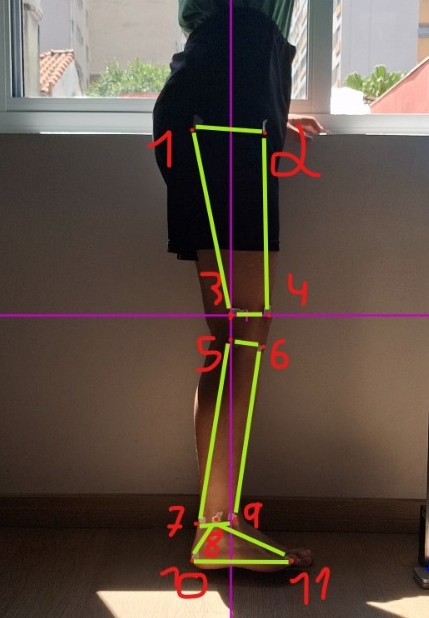
\includegraphics[width=0.36\textwidth]{figuras/rasc_p6_0.jpeg}
  \caption{Geometria adotada para a representação do membro inferior.}
  \label{fig:geometria}
\end{figure}

Na representação adotada, os pontos 1 e 2 estão localizados na região do quadril,
enquanto os pontos 3 e 4 estão posicionados na extremidade inferior da coxa, próxima à
região do joelho. Para a perna, os pontos 5 e 6 estão localizados imediatamente abaixo
do joelho, enquanto os pontos 7 e 9 estão posicionados aproximadamente na região do
tornozelo. O ponto 8 está localizado entre os pontos 7 e 9, contribuindo para a
representação da conexão entre a perna e o pé. Por fim, os pontos 10 e 11 correspondem
às extremidades inferiores da representação do pé.

A escolha de um mecanismo quadrilátero articulado para representar o movimento do
joelho está relacionada à necessidade de reproduzir adequadamente o movimento relativo
observado entre a coxa e a perna. Uma representação mais simples, na qual a coxa e a
perna fossem consideradas elementos rígidos conectados diretamente por uma única junta
de revolução, permitiria descrever apenas uma rotação da perna em torno de um centro
fixo. Nesse caso, os pontos pertencentes à perna descreveriam trajetórias circulares em
relação à coxa, o que constitui uma aproximação limitada do movimento do joelho.

O emprego de um quadrilátero articulado permite obter o movimento relativo entre a
coxa e a perna a partir da combinação das rotações de seus diferentes elos. Dessa
forma, o centro instantâneo do movimento relativo entre os segmentos (o polo $I_{13}$ da
\cref{sec:cadeia_fechada}) pode variar durante a movimentação, permitindo reproduzir
trajetórias mais complexas do que aquelas obtidas por uma única junta de revolução.
Essa característica é particularmente relevante para o problema proposto, uma vez que
o movimento relativo entre a coxa e a perna não pode ser rigorosamente representado
apenas por uma junta de rotação.

A representação do pé por meio de uma geometria triangular foi adotada de maneira
análoga, buscando preservar sua extensão e sua orientação em relação à perna. Uma
representação por um único elemento rígido poderia descrever apenas a distância entre
dois pontos, sem representar simultaneamente diferentes pontos de referência
associados ao pé. A geometria triangular fornece, portanto, uma representação rígida
simplificada da região, possibilitando acompanhar sua posição e orientação durante o
movimento.

Embora os pontos utilizados na aquisição experimental tenham sido definidos próximos
aos vértices das regiões utilizadas na representação geométrica, a localização das
articulações do mecanismo não está necessariamente restrita a esses pontos
experimentais. Articulações localizadas no interior das regiões correspondentes à coxa
e à perna também podem ser consideradas durante a síntese, desde que sejam compatíveis
com a geometria e com o movimento desejado.

\subsection{Aquisição experimental do movimento}\label{sec:aquisicao}

Após a definição da geometria, foram realizadas medições experimentais com o objetivo
de obter as posições dos pontos de interesse ao longo do movimento do membro inferior.
Para isso, um integrante do grupo realizou o movimento com a própria perna, e foi
registrada uma sequência de vídeo com o membro observado lateralmente.

Foram consideradas três configurações principais para caracterizar o movimento. A
configuração inicial corresponde à posição em pé, na qual a coxa, a perna e o pé se
encontram aproximadamente alinhados. A configuração intermediária corresponde a uma
flexão da perna de aproximadamente \SI{90}{\degree} em relação à coxa, mantendo-se a
posição da coxa. Por fim, a configuração final corresponde à condição de maior flexão
observada durante o experimento, na qual a perna se aproxima da coxa. A sequência de
configurações observada durante o movimento é apresentada na \cref{fig:sequencia}.

\begin{figure}[htbp]
  \centering
  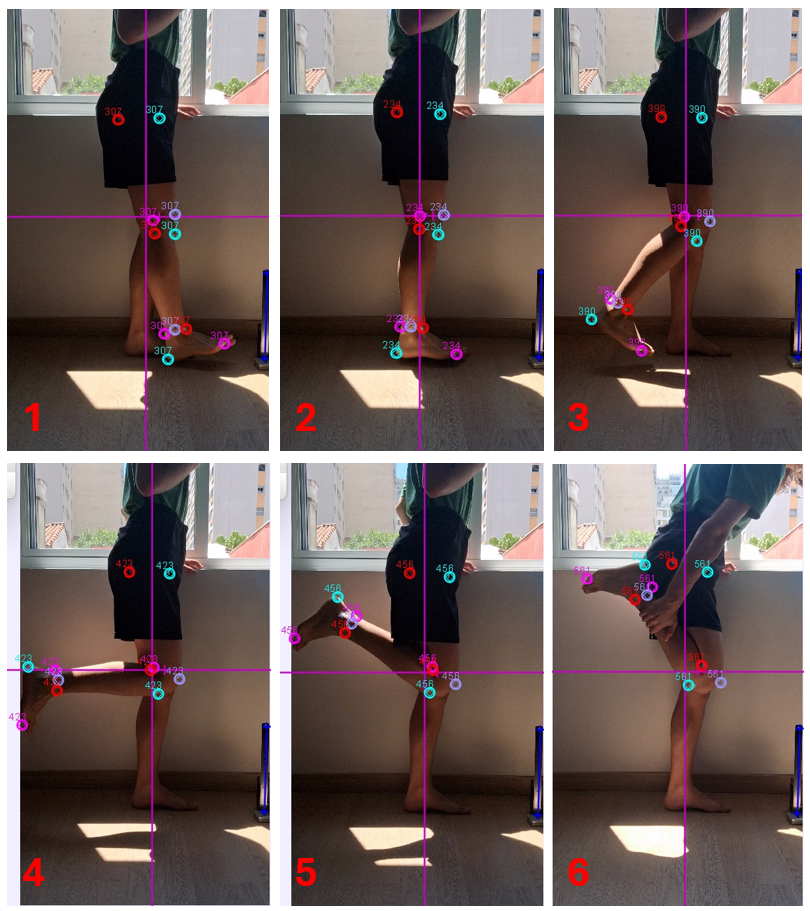
\includegraphics[width=0.62\textwidth]{figuras/rasc_p7_0.png}
  \caption{Sequência de configurações do membro inferior durante o movimento experimental.}
  \label{fig:sequencia}
\end{figure}

Para o processamento do vídeo foi empregado o software \emph{Tracker} \cite{tracker},
que permite acompanhar a posição de pontos específicos ao longo dos diferentes
\emph{frames} de uma gravação. Foram definidos pontos de referência próximos aos
vértices das regiões utilizadas na representação geométrica da coxa, da perna e do pé.
Esses pontos foram identificados e acompanhados individualmente ao longo do movimento,
permitindo obter suas coordenadas no plano da imagem em função do tempo. A numeração
dos pontos utilizada no rastreamento corresponde à geometria apresentada anteriormente
(\cref{fig:geometria}).

\begin{figure}[htbp]
  \centering
  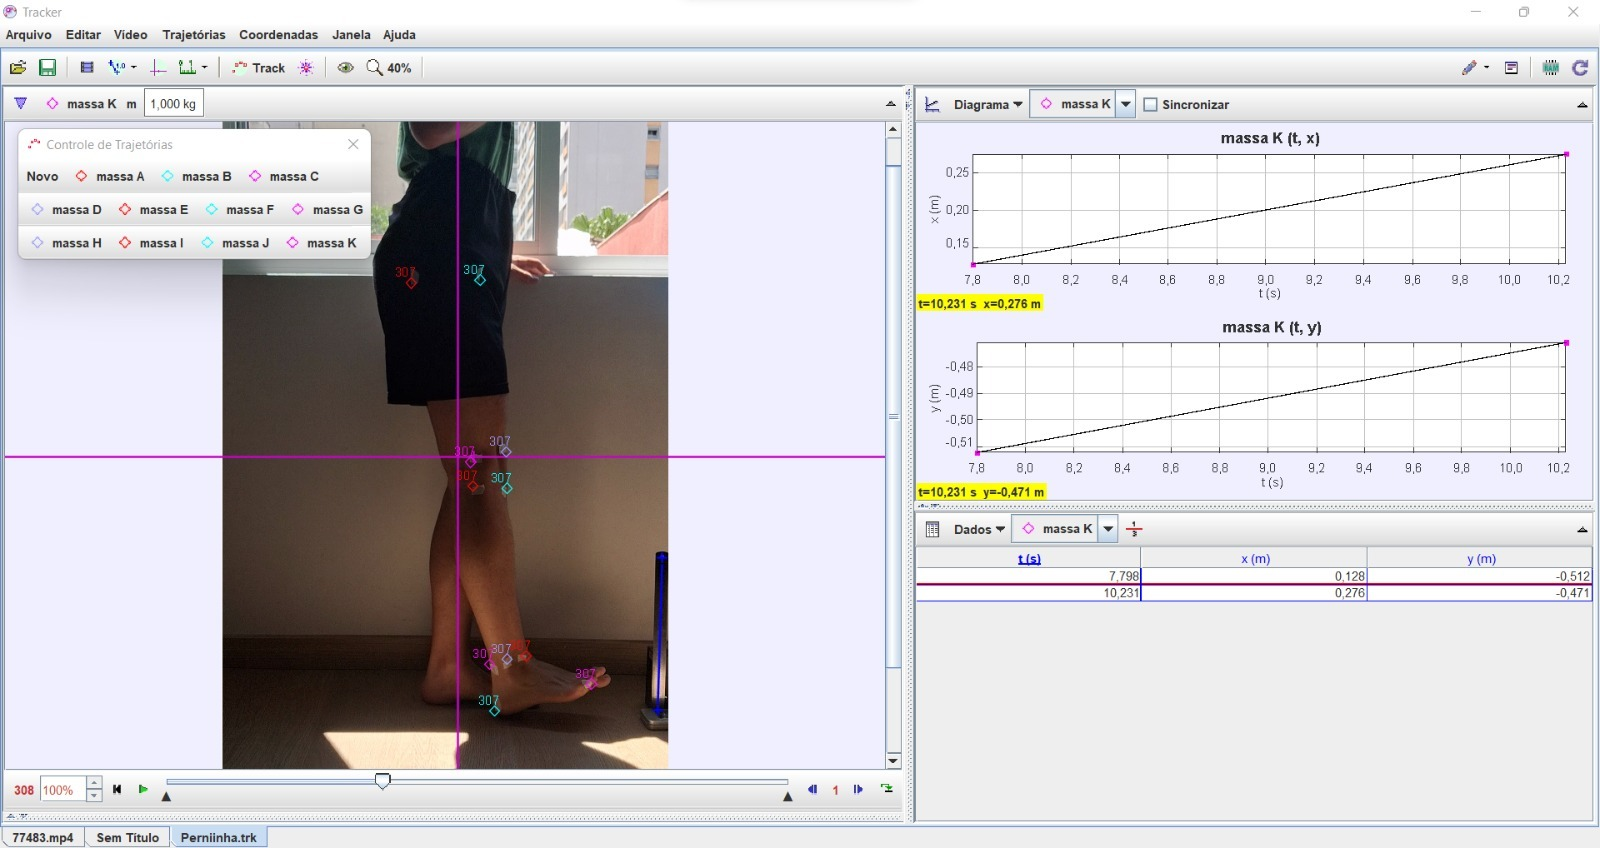
\includegraphics[width=\textwidth]{figuras/rasc_p8_0.jpeg}
  \caption{Rastreamento dos pontos do membro inferior e obtenção das posições no software \emph{Tracker}.}
  \label{fig:tracker}
\end{figure}

A partir do rastreamento, o \emph{Tracker} forneceu as coordenadas $x$ e $y$ dos pontos
acompanhados para os diferentes instantes analisados. Os valores obtidos correspondem,
portanto, às posições dos pontos no plano da imagem (base $im$, com a escala calibrada
em metros), e não diretamente aos comprimentos dos elos do mecanismo. O software também
permitiu visualizar graficamente a evolução temporal dessas coordenadas.

A planilha de dados obtida a partir do rastreamento contém as coordenadas dos onze
pontos para os \emph{frames} 234, 307, 390, 423, 456 e 561 (\cref{tab:tracker}, na
\cref{sec:anexos}). Para a análise do movimento, foram usados os \emph{frames}
234, 307, 390, 423 e 456, todos dentro da faixa de flexão de interesse. O \emph{frame} 561
foi desconsiderado, pois corresponde a uma etapa do movimento em que houve auxílio manual
para conduzir a perna (os marcadores da coxa se deslocaram em relação aos do quadril).

\subsection{Processamento dos dados e posições de precisão}\label{sec:processamento}

As coordenadas do \emph{Tracker} estão na base da imagem. O que interessa ao
quadrilátero do joelho é apenas o movimento \emph{relativo} entre a coxa e a perna; por
isso, o movimento angular do quadril (a rotação da coxa em relação ao tronco, que
também ocorre levemente durante o experimento) foi desconsiderado, e a coxa foi tratada
como o elo fixo do mecanismo. Os dados foram processados em quatro passos.

\paragraph{1º passo -- base da coxa em cada quadro.} A base $0$ tem origem no ponto médio
dos marcadores 3 e 4 (extremidade distal da coxa, junto ao joelho) e eixos paralelos aos
da imagem: $X_0$ horizontal, para a frente, e $Y_0$ vertical, para cima. Como a rotação
do quadril é desconsiderada, $\Rm{im}{0} = \Rot{0}{z_0} = I$, e a base da coxa apenas
acompanha a translação da região do joelho entre os quadros. Com
$\rv{im}{O_0} = \tfrac12\big(\rv{im}{3} + \rv{im}{4}\big)$, a mudança de base inversa de
\eqref{eq:mudancabase} fornece as coordenadas de cada marcador $k$ na base da coxa:
\begin{equation}
  \rv{0}{k} = \Rm{im}{0}^{\mathsf T}\big(\rv{im}{k} - \rv{im}{O_0}\big) = \rv{im}{k} - \tfrac12\big(\rv{im}{3} + \rv{im}{4}\big).
\end{equation}
Os marcadores 1 e 2 (quadril) não entram na síntese da Parte~I. Para referência, se a
rotação da coxa fosse descontada (eixo definido pelos pontos médios 1--2 e 3--4), as
flexões mudariam de cerca de \SI{5}{\degree}, porque a coxa girou apenas alguns graus durante
o experimento.

\paragraph{2º passo -- pose da perna.} A perna é tratada como corpo rígido definido por dois
pontos (\cref{sec:pose2pontos}): $J$, ponto médio dos marcadores 5 e 6 (logo abaixo do
joelho), e $P$, marcador 8 (conexão perna--pé, tornozelo). A base $4$ é presa à perna com
origem em $J$ e, no quadro \frRef{} (membro estendido), eixos paralelos aos da base $0$, de
modo que $\Rm{0}{4}^{(\frRef)} = I$, $\rv{0}{J}^{(\frRef)} = [\Jx\ \ \Jy]^{\mathsf T}$~mm e
$\rv{4}{P} = \rv{0}{P}^{(\frRef)} - \rv{0}{J}^{(\frRef)} = [\Px\ \ \Py]^{\mathsf T}$~mm. Em cada quadro obtêm-se
$\alpha_j$ e $\rv{0}{O_4}^{(j)} = \rv{0}{J}^{(j)}$; a flexão do joelho é $\varphi_j = -\alpha_j$.

\paragraph{3º passo -- tornozelo.} A posição do tornozelo segundo o modelo rígido é
$\rv{0}{P}^{(j)} = \Rm{0}{4}^{(j)}\,\rv{4}{P} + \rv{0}{O_4}^{(j)}$; é essa posição que será comparada com a
gerada pelo mecanismo.

\paragraph{4º passo -- suavização por mínimos quadrados.} As poses medidas contêm erros de
alguns milímetros (marcação manual e deslizamento da pele sobre os ossos). Em vez de impor ao
mecanismo pontos com esse ruído, a trajetória de $J$ foi ajustada por um polinômio de 2º grau
em função da flexão, ${}^0x_J(\varphi) = a_0 + a_1\varphi + a_2\varphi^2$ (e o mesmo para
${}^0y_J$, com coeficientes $b_k$). Com os $m = 5$ quadros medidos, em forma matricial,
\begin{equation}
  [A] = \begin{bmatrix} 1 & \varphi_1 & \varphi_1^2 \\ \vdots & \vdots & \vdots \\ 1 & \varphi_m & \varphi_m^2 \end{bmatrix},
  \qquad
  [A]^{\mathsf T}[A]\,\mathbf a = [A]^{\mathsf T}\,\mathbf x_J ,
  \qquad
  [A]^{\mathsf T}[A]\,\mathbf b = [A]^{\mathsf T}\,\mathbf y_J ,
  \label{eq:minquad}
\end{equation}
em que $\mathbf x_J$ e $\mathbf y_J$ reúnem as coordenadas medidas. São três equações para três
incógnitas, resolvidas como um sistema linear comum. Obtiveram-se
$\mathbf a = [\cxZero\ \ \cxUm\ \ \cxDois]^{\mathsf T}$ e $\mathbf b = [\cyZero\ \ \cyUm\ \ \cyDois]^{\mathsf T}$
(mm e graus), com resíduos de no máximo \resmax~mm (\cref{fig:ajuste}), da ordem da incerteza
das medições. A pose ajustada em qualquer flexão é então
$\Rm{0}{4}(\varphi) = \Rot{-\varphi}{z_4}$ e $\rv{0}{O_4}(\varphi) = [{}^0x_J(\varphi)\ \ {}^0y_J(\varphi)]^{\mathsf T}$, e é sobre
essa trajetória suavizada que se escolhem as posições de precisão. Os pontos medidos
continuam sendo usados para verificar o resultado.

\begin{figure}[htbp]
  \centering
  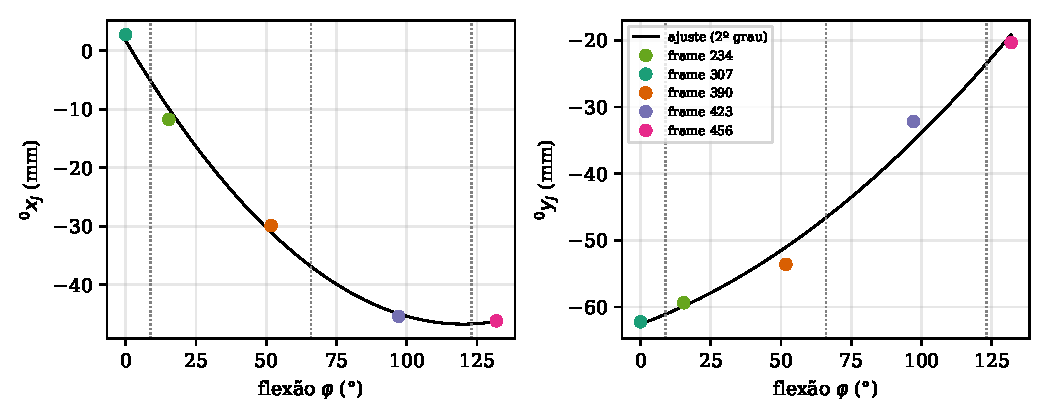
\includegraphics[width=0.95\textwidth]{figuras/p1_ajuste.pdf}
  \caption{Coordenadas medidas de $J$ na base da coxa e ajuste de 2º grau por mínimos
  quadrados (linhas pontilhadas: flexões das posições de precisão).}
  \label{fig:ajuste}
\end{figure}

\begin{table}[htbp]
  \centering
  \caption{Poses da perna na base $0$ (coxa) obtidas das medições (mm). $\dagger$: quadro não
  utilizado. $\overline{JP}$: comprimento medido entre os pontos $J$ e $P$; $r$: resíduo do
  ajuste em $J$; $e$: distância entre o tornozelo do mecanismo sintetizado e o medido.}
  \label{tab:poses}
  \small
  \begin{tabular}{lrrrrrrrr}
    \toprule
    Quadro & $\varphi$ (\si{\degree}) & ${}^0x_{J}$ & ${}^0y_{J}$ & ${}^0x_{P}$ & ${}^0y_{P}$ & $\overline{JP}$ & $r$ & $e$ \\
    \midrule
    \tabelaposes
    \bottomrule
  \end{tabular}
\end{table}

\begin{figure}[htbp]
  \centering
  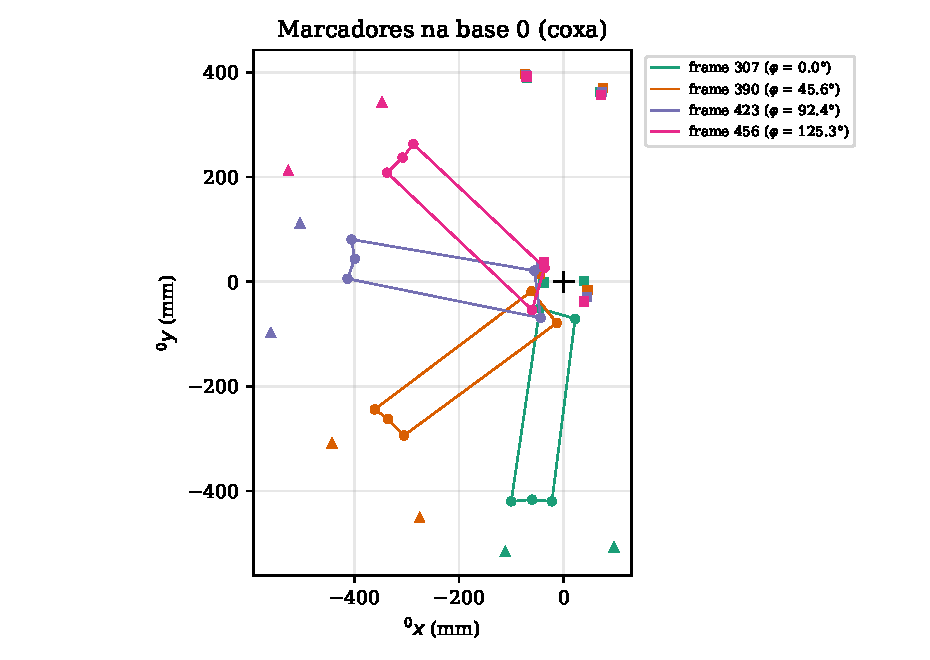
\includegraphics[width=0.85\textwidth]{figuras/p1_medicoes.pdf}
  \caption{Marcadores dos quadros selecionados escritos na base da coxa, com origem entre os pontos 3 e 4 ($\square$: coxa,
  $\circ$: perna, $\triangle$: pé; linha: segmento $JP$).}
  \label{fig:medicoes}
\end{figure}

Os quadros utilizados correspondem a flexões de \phiB, \phiA, \phiC, \phiD{} e
\phiE\si{\degree} (\cref{tab:poses,fig:medicoes}), da extensão completa à máxima
flexão. O comprimento $\overline{JP}$ varia entre \JPmin{} e \JPmax~mm (cerca de
\SI{\JPvar}{\percent}), o que mede a incerteza da marcação manual e dos artefatos de pele.
Nota-se também que, além de girar, a perna se desloca: o ponto $J$ muda de posição em até
cerca de \SI{\deslO}{mm} na base da coxa durante o movimento:
esse é justamente o efeito que uma junta de revolução simples não reproduz e que motiva
o uso do quadrilátero.

\paragraph{Escolha das posições de precisão.} As três posições de precisão são tomadas
sobre a trajetória ajustada, entre \SI{0}{\degree} e a maior flexão medida, \phimax\si{\degree}.
Foram comparadas duas escolhas (\cref{tab:combos}): posições igualmente espaçadas e o
espaçamento de Chebyshev (\cref{eq:chebyshev}). Adotou-se a de menor erro,
$\varphi_1 = \precphiA$, $\varphi_2 = \precphiB$ e $\varphi_3 = \precphiC\si{\degree}$ (Chebyshev).

\begin{table}[htbp]
  \centering
  \caption{Escolhas de posições de precisão testadas. $e_{\max}$: maior distância entre o
  tornozelo do mecanismo e o da trajetória ajustada em toda a faixa; $e_{\mathrm{med}}$: maior
  distância ao tornozelo medido nos cinco quadros; $\mu_{\min}$: menor ângulo nas articulações
  móveis.}
  \label{tab:combos}
  \begin{tabular}{lcccc}
    \toprule
    Espaçamento & $\varphi_1;\ \varphi_2;\ \varphi_3$ (\si{\degree}) & $e_{\max}$ (mm) & $e_{\mathrm{med}}$ (mm) & $\mu_{\min}$ (\si{\degree}) \\
    \midrule
    \tabelacombos
    \bottomrule
  \end{tabular}
\end{table}

\subsection{Determinação das escolhas livres}\label{sec:escolha}

Cada díade tem duas escolhas livres (\cref{sec:diade}), $(\beta_2, \beta_3)$ para $CQ$ e
$(\gamma_2, \gamma_3)$ para $LN$. Elas foram determinadas por varredura, em quatro passos:
\begin{enumerate}
  \item para cada díade, $\beta_2$ e $\beta_3$ percorrem de \SI{-180}{\degree} a \SI{180}{\degree} em passos
  de \SI{4}{\degree}; para cada par, $\mathbf W$ e $\mathbf Z$ são calculados pela \cref{eq:cramer};
  \item descartam-se as díades cujo pivô fixo cai fora da região do joelho
  ($|{}^0x| \le \SI{60}{mm}$, $\SI{-40}{mm} \le {}^0y \le \SI{60}{mm}$), cujo pivô móvel cai fora da
  parte proximal da perna ($|{}^4x| \le \SI{60}{mm}$, $|{}^4y| \le \SI{60}{mm}$, em torno de $J$) ou
  cujo comprimento $|\mathbf W|$ não está entre \SI{20}{mm} e \SI{120}{mm};
  \item todas as díades restantes são combinadas duas a duas ($CQ$ com $LN$); para cada par, o
  mecanismo é montado por Newton--Raphson (\cref{eq:newton}) de \SI{0}{\degree} até a flexão
  máxima medida, e descartam-se os que mudam de ramo, atingem ponto morto ou têm
  $\mu_N < \SI{30}{\degree}$ ou $\mu_Q < \SI{30}{\degree}$ em algum ponto da faixa (barras quase
  alinhadas);
  \item para cada mecanismo restante, calcula-se o maior erro no tornozelo em relação à
  trajetória ajustada,
  \begin{equation}
    e_{\max} = \max_{0 \le \varphi \le \varphi_{\max}} \Big\lVert \rv{0}{P}^{\,\mathrm{mec}}(\varphi) - \rv{0}{P}^{\,\mathrm{aj}}(\varphi) \Big\rVert ,
  \end{equation}
  e escolhe-se o de menor $e_{\max}$ (abaixo de \SI{1}{mm}, prefere-se o de maior ângulo mínimo);
  a varredura é então refinada com passo de \SI{0,5}{\degree} em torno das escolhas encontradas.
\end{enumerate}

\section{Parte I -- Resultados da síntese}\label{cap:resultados1}

\subsection{Mecanismo sintetizado}

A \cref{tab:diade} apresenta os dados das posições de precisão, as escolhas livres adotadas e
os vetores das díades obtidos pela \cref{eq:cramer}; a \cref{tab:pivos} apresenta os pivôs e
os comprimentos resultantes.

\begin{table}[htbp]
  \centering
  \caption{Síntese pela díade padrão: dados, escolhas livres e solução (mm e graus).}
  \label{tab:diade}
  \begin{tabular}{lll}
    \toprule
    & Ângulos (\si{\degree}) & Vetores (mm) \\
    \midrule
    Dados ($\varphi_1 = \precphiA$) & & $\rv{0}{O_4}^{(1)} = [\dOx\ \ \dOy]^{\mathsf T}$ \\
    Dados ($\varphi_2 = \precphiB$, $\varphi_3 = \precphiC$) & $\alpha_2 = \dalphaA$ & $\boldsymbol\delta_2 = [\ddeltaAx\ \ \ddeltaAy]^{\mathsf T}$ \\
                                            & $\alpha_3 = \dalphaB$ & $\boldsymbol\delta_3 = [\ddeltaBx\ \ \ddeltaBy]^{\mathsf T}$ \\
    \midrule
    Díade $CQ$ (escolhas livres) & $\beta_2 = \dbetaA$ & $\mathbf W = [\dWx\ \ \dWy]^{\mathsf T}$ \\
                                  & $\beta_3 = \dbetaB$ & $\mathbf Z = [\dZx\ \ \dZy]^{\mathsf T}$ \\
    \midrule
    Díade $LN$ (escolhas livres) & $\gamma_2 = \dgamA$ & $\mathbf U = [\dUx\ \ \dUy]^{\mathsf T}$ \\
                                  & $\gamma_3 = \dgamB$ & $\mathbf S = [\dSx\ \ \dSy]^{\mathsf T}$ \\
    \bottomrule
  \end{tabular}
\end{table}

\begin{table}[htbp]
  \centering
  \caption{Pivôs e comprimentos do quadrilátero sintetizado (mm).}
  \label{tab:pivos}
  \begin{tabular}{lll}
    \toprule
    Articulação & Elo & Coordenadas \\
    \midrule
    $C$ & coxa (fixo) & $\rv{0}{C} = [\Cx\ \ \Cy]^{\mathsf T}$ \\
    $L$ & coxa (fixo) & $\rv{0}{L} = [\Lx\ \ \Ly]^{\mathsf T}$ \\
    $Q$ & perna (móvel) & $\rv{4}{Q} = [\Qx\ \ \Qy]^{\mathsf T}$ \\
    $N$ & perna (móvel) & $\rv{4}{N} = [\Nx\ \ \Ny]^{\mathsf T}$ \\
    \midrule
    \multicolumn{3}{l}{Comprimentos: $\ell_0 = \overline{CL} = \rCL$, $\ell_1 = \overline{CQ} = \rCQ$, $\ell_2 = \overline{QN} = \rQN$, $\ell_3 = \overline{LN} = \rLN$} \\
    \bottomrule
  \end{tabular}
\end{table}

\paragraph{Grashof.} Com $s=\grashofs$, $p=\grashofp$, $q=\grashofq$ e $l=\grashofl$~mm,
$s+l=\grashofsl \grashofsinal p+q=\grashofpq$: o mecanismo \grashof{} a condição
\eqref{eq:grashof}, o que não é um problema, pois o joelho só precisa percorrer a faixa de
flexão medida. A simulação de montagem confirma que ele percorre continuamente a faixa de
\SI{0}{\degree} a \phimax\si{\degree} sem atingir pontos mortos, com $\mu_N$ entre
\mumin\si{\degree} e \mumax\si{\degree} e $\mu_Q$ entre \muQmin\si{\degree} e
\muQmax\si{\degree} (\cref{fig:erro}): nenhuma das articulações móveis se aproxima do
alinhamento, e o quadrilátero (cruzado, como em muitos joelhos policêntricos) não se dobra
sobre si mesmo.

\paragraph{Precisão.} Nas três posições de precisão o erro em relação à trajetória ajustada é
nulo (a menos da tolerância numérica), como esperado, e em toda a faixa ele não passa de
$e_{\max} = \ecurva$~mm. Em relação aos cinco quadros medidos, o tornozelo do mecanismo fica
entre \emedmin{} e \emedmax~mm do tornozelo medido (\cref{tab:poses}), valores da ordem dos
resíduos do próprio ajuste e inferiores à incerteza das medições (a variação de
$\overline{JP}$ entre os quadros é de \JPmin{} a \JPmax~mm). O mecanismo reproduz, portanto, o
movimento medido dentro da incerteza experimental. A \cref{fig:mecanismo} mostra o
mecanismo nos cinco quadros medidos, a centroide (trajetória do polo $I_{13}$) e a
trajetória do tornozelo.

\begin{figure}[htbp]
  \centering
  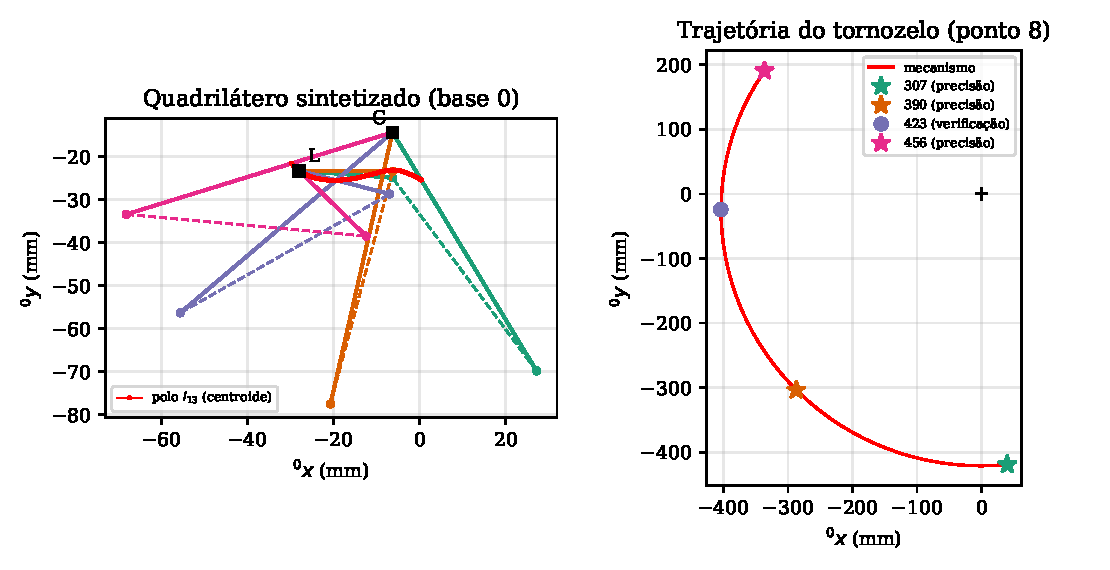
\includegraphics[width=\textwidth]{figuras/p1_mecanismo.pdf}
  \caption{Esquerda: quadrilátero sintetizado nos cinco quadros medidos (tracejado:
  acoplador $QN$) e centroide. Direita: trajetória do tornozelo gerada pelo mecanismo, trajetória
  ajustada, posições de precisão ($\star$) e posições medidas.}
  \label{fig:mecanismo}
\end{figure}

\begin{figure}[htbp]
  \centering
  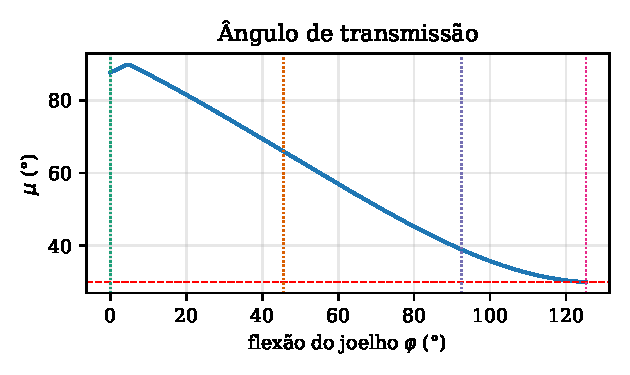
\includegraphics[width=0.6\textwidth]{figuras/p1_erro_mu.pdf}
  \caption{Ângulos nas articulações móveis em função da flexão (linhas verticais: quadros medidos).}
  \label{fig:erro}
\end{figure}

\subsection{Discussão}

Os ângulos nas duas articulações móveis permanecem acima de \mumindois\si{\degree} em toda
a faixa, respeitando o limite de \SI{30}{\degree} imposto na escolha das escolhas livres, de
modo que a transmissão de forças é boa e as barras nunca ficam alinhadas. Os pivôs fixos ficam na
região da articulação do joelho e os móveis, na parte proximal da perna, com elos entre
\rminelo{} e \rmaxelo~mm. O polo parte de
$(\ciOx;\ \ciOy)$~mm na extensão e migra posteriormente até $(\ciFx;\ \ciFy)$~mm na
flexão máxima, comportamento qualitativamente semelhante à centroide em ``J'' descrita
por \textcite{oconnor1989}. A suavização por mínimos quadrados e o espaçamento de Chebyshev
foram decisivos: com as poses medidas usadas diretamente como posições de precisão, o ruído
das medições restringia muito as soluções e o erro na verificação era maior. Como a
incerteza das medições é de alguns milímetros, o refinamento natural do projeto é repetir a
medição com mais quadros do vídeo, o que melhora o ajuste. Para uma prótese transfemoral real, recomenda-se ainda verificar a posição
do polo em extensão em relação à linha trocânter--joelho--tornozelo, da qual depende a
estabilidade voluntária na fase de apoio \cite{radcliffe1994}.

\subsection{Maquete}\label{cap:maquete}

\section{Conclusões}

\begin{itemize}
  \item \textbf{Parte I}: as medições feitas com o \emph{Tracker} foram escritas na base da
  coxa, desconsiderando o movimento angular do quadril, e a perna foi tratada como corpo
  rígido definido por dois pontos, fornecendo cinco poses entre \SI{0}{\degree} e
  \phiE\si{\degree} de flexão, suavizadas por mínimos quadrados. A síntese do tipo levou ao
  quadrilátero articulado, e a síntese dimensional analítica pela equação da díade padrão,
  com posições de precisão em espaçamento de Chebyshev e escolhas livres determinadas por
  varredura, produziu um mecanismo compacto (elos de \rminelo{} a \rmaxelo~mm) que segue o
  movimento ajustado com erro máximo de \ecurva~mm e fica a no máximo \emedmax~mm dos
  tornozelos medidos. A análise de posição por Newton--Raphson mostra que o mecanismo
  percorre toda a faixa medida sem pontos mortos, com ângulos de pelo menos
  \mumindois\si{\degree} nas duas articulações móveis.
  \item \textbf{Próximos passos}: construir e ensaiar a maquete, refinar a síntese com mais
  quadros do vídeo e realizar a Parte~II (órtese).
\end{itemize}

\section{Materiais e anexos}\label{sec:anexos}

Os arquivos utilizados na aquisição e no tratamento dos dados experimentais são
disponibilizados juntamente com o relatório, incluindo o arquivo do projeto utilizado
no software \emph{Tracker}, a planilha com as coordenadas obtidas durante o rastreamento
e os programas em Python usados na análise.

\subsection{Dados experimentais obtidos pelo \emph{Tracker}}

A tabela a seguir apresenta as coordenadas cartesianas dos onze pontos rastreados para os
\emph{frames} registrados durante o experimento. Os valores correspondem diretamente aos
dados obtidos no arquivo de saída utilizado para a organização dos resultados
experimentais.

{\small
\begin{longtable}{cc rr}
  \caption{Coordenadas dos pontos obtidas pelo \emph{Tracker}.}\label{tab:tracker}\\
  \toprule
  Frame & Ponto & $x$ (m) & $y$ (m) \\
  \midrule
  \endfirsthead
  \toprule
  Frame & Ponto & $x$ (m) & $y$ (m) \\
  \midrule
  \endhead
  \midrule
  \multicolumn{4}{r}{Continua na próxima página}\\
  \endfoot
  \bottomrule
  \endlastfoot
    234 & 1 & \ensuremath{-}0.078146 & 0.386447 \\
    234 & 2 & 0.069715 & 0.381067 \\
    234 & 3 & 0.000380 & 0.000035 \\
    234 & 4 & 0.084056 & 0.004970 \\
    234 & 5 & \ensuremath{-}0.003477 & \ensuremath{-}0.046264 \\
    234 & 6 & 0.064449 & \ensuremath{-}0.067460 \\
    234 & 7 & \ensuremath{-}0.067107 & \ensuremath{-}0.412356 \\
    234 & 8 & \ensuremath{-}0.028615 & \ensuremath{-}0.411334 \\
    234 & 9 & 0.010899 & \ensuremath{-}0.415762 \\
    234 & 10 & \ensuremath{-}0.081579 & \ensuremath{-}0.508887 \\
    234 & 11 & 0.128059 & \ensuremath{-}0.512169 \\
    307 & 1 & \ensuremath{-}0.096598 & 0.361130 \\
    307 & 2 & 0.045186 & 0.368099 \\
    307 & 3 & 0.025422 & \ensuremath{-}0.010538 \\
    307 & 4 & 0.100385 & 0.010706 \\
    307 & 5 & 0.030582 & \ensuremath{-}0.060615 \\
    307 & 6 & 0.100689 & \ensuremath{-}0.063650 \\
    307 & 7 & 0.064449 & \ensuremath{-}0.431417 \\
    307 & 8 & 0.102506 & \ensuremath{-}0.418892 \\
    307 & 9 & 0.140082 & \ensuremath{-}0.413111 \\
    307 & 10 & 0.076024 & \ensuremath{-}0.527587 \\
    307 & 11 & 0.276455 & \ensuremath{-}0.470734 \\
    390 & 1 & \ensuremath{-}0.092092 & 0.369497 \\
    390 & 2 & 0.059443 & 0.364994 \\
    390 & 3 & \ensuremath{-}0.006151 & \ensuremath{-}0.003193 \\
    390 & 4 & 0.087942 & \ensuremath{-}0.021160 \\
    390 & 5 & \ensuremath{-}0.017371 & \ensuremath{-}0.039370 \\
    390 & 6 & 0.039383 & \ensuremath{-}0.092178 \\
    390 & 7 & \ensuremath{-}0.279894 & \ensuremath{-}0.307356 \\
    390 & 8 & \ensuremath{-}0.252276 & \ensuremath{-}0.321620 \\
    390 & 9 & \ensuremath{-}0.217070 & \ensuremath{-}0.348328 \\
    390 & 10 & \ensuremath{-}0.350911 & \ensuremath{-}0.384140 \\
    390 & 11 & \ensuremath{-}0.164262 & \ensuremath{-}0.499468 \\
    423 & 1 & \ensuremath{-}0.084368 & 0.364992 \\
    423 & 2 & 0.064305 & 0.358922 \\
    423 & 3 & 0.005695 & 0.010403 \\
    423 & 4 & 0.101903 & \ensuremath{-}0.032390 \\
    423 & 5 & \ensuremath{-}0.005007 & 0.000303 \\
    423 & 6 & 0.021836 & \ensuremath{-}0.086645 \\
    423 & 7 & \ensuremath{-}0.359654 & 0.000097 \\
    423 & 8 & \ensuremath{-}0.347216 & \ensuremath{-}0.035323 \\
    423 & 9 & \ensuremath{-}0.354246 & \ensuremath{-}0.075069 \\
    423 & 10 & \ensuremath{-}0.461318 & 0.013346 \\
    423 & 11 & \ensuremath{-}0.481342 & \ensuremath{-}0.202402 \\
    456 & 1 & \ensuremath{-}0.055404 & 0.367781 \\
    456 & 2 & 0.090948 & 0.353055 \\
    456 & 3 & 0.026919 & 0.021650 \\
    456 & 4 & 0.113090 & \ensuremath{-}0.042424 \\
    456 & 5 & 0.029978 & 0.010953 \\
    456 & 6 & 0.017711 & \ensuremath{-}0.072400 \\
    456 & 7 & \ensuremath{-}0.251153 & 0.209797 \\
    456 & 8 & \ensuremath{-}0.267954 & 0.181360 \\
    456 & 9 & \ensuremath{-}0.293245 & 0.148842 \\
    456 & 10 & \ensuremath{-}0.321909 & 0.280117 \\
    456 & 11 & \ensuremath{-}0.480643 & 0.126200 \\
    561 & 1 & \ensuremath{-}0.047680 & 0.402324 \\
    561 & 2 & 0.081961 & 0.370923 \\
    561 & 3 & 0.061252 & 0.027057 \\
    561 & 4 & 0.131913 & \ensuremath{-}0.038073 \\
    561 & 5 & 0.061220 & 0.026248 \\
    561 & 6 & 0.013809 & \ensuremath{-}0.047533 \\
    561 & 7 & \ensuremath{-}0.122496 & 0.315720 \\
    561 & 8 & \ensuremath{-}0.138852 & 0.285733 \\
    561 & 9 & \ensuremath{-}0.185196 & 0.271421 \\
    561 & 10 & \ensuremath{-}0.149757 & 0.399547 \\
    561 & 11 & \ensuremath{-}0.363074 & 0.346388 \\
\end{longtable}
}

\subsection{Programas}\label{ap:codigo}



Os programas estão na pasta \texttt{scripts/} e são executados pelo \texttt{Makefile}
(\texttt{make}), que regenera figuras, tabelas e o PDF.

\begin{description}
  \item[\texttt{parte1\_sintese.py}] leitura dos dados do \emph{Tracker}; base da coxa e poses
  da perna por dois pontos; síntese pela díade padrão (regra de Cramer) com varredura das
  escolhas livres; análise de posição por Newton--Raphson;
  erro na verificação, ângulo de transmissão e centroide.
  \item[\texttt{gera\_valores\_tex.py}] exporta os resultados para \texttt{dados/valores.tex}.
\end{description}




\clearpage
\printbibliography[heading=bibintoc,title={Referências}]

\end{document}
